\section{How common are sign flips?} 
\label{sec:signflips}

Our examples above serve as existence proofs that conclusion reversals are possible when using the OBD with different references.
In what follows, we focus on conclusions based on sign flips.
We show that sign reversals (of either the explained or unexplained component) represent a large proportion of the parameter space, in a sense we make precise below.
Then we explain why these sign flips still might not be common in practical applications.

\subsection{Signed conclusions}

We start by concretizing the type of decision we will focus on in our analysis. 
In particular, we will consider a conclusion based on the sign of either the explained or unexplained component of the OBD.
We will assume we are working with full population information so that a sign flip alone is enough to change conclusions;
when working with finite samples (as will always be the case in practice), we might also be concerned with statistical significance.
Although flipping from a signed value to zero could also be considered to change conclusions, we here focus on the more
extreme case where we able to flip to the opposite sign by choosing a different reference.

\textbf{Explained component.}
Recall from \cref{eq:ob_decomp_ref_group} the two possible explained components, each corresponding to a different reference.
With this notation in hand, we can define changing a signed conclusion at the population level.
\begin{definition}
	We say the OBD \emph{sign flips the explained component} if the sign of the explained term, $\Delta\mu^T \beta_g$, depends on the reference group. That is,
	\begin{equation}
        \label{eq:sign_flip_condition_explained_neq}
		\sign\!\left(\Delta\mu^T \beta_H\right) \neq \sign\!\left(\Delta\mu^T \beta_K\right).
	\end{equation}
\end{definition}

From the definition, we can immediately see the following alternative characterization.
%
\begin{remark}
    \label{rmk:explained_ordering_sensitivity}
    The OBD sign flips the explained component if and only if the following two conditions hold:
    \begin{gather}
    	\nonumber
    	\Delta\mu^T \beta_H \neq \Delta\mu^T \beta_K \\
    \label{eq:sign_flip_condition_explained}
        \min\{\Delta\mu^T \beta_H,\ \Delta\mu^T \beta_K\}
        < 0 <
        \max\{\Delta\mu^T \beta_H,\ \Delta\mu^T \beta_K\}.
    \end{gather}
\end{remark}
Since $\Delta\mu$ is constant across analyses, sign flips in the explained component are straightforwardly driven
by differences in sign in the slope between groups.

% A large region of the parameter space satisfies \cref{eq:sign_flip_condition_explained_neq}.
% We compute the volume of this region by integrating the region that satsfies \cref{eq:sign_flip_condition_explained_neq} against a Uniform(-M, M) measure on \( \beta_H \) and \( \beta_K \), where \( M \) is large.
% The computations, which appear in \cref{app:sign_flip_volume}, show that 50\% of the parameter space satisfies \cref{eq:sign_flip_condition_explained_neq}.

%To see how this characterization applies in practice, we return to the ICU mortality and heart rate example presented in \cref{sec:real_example}. In that example, we observed a sign flip in the explained component of the OBD when using men or women as the reference group. Within HR quartile two, the covariate mean difference $\Delta\mu$ between men and women is fixed by the sample, but the coefficients governing how mortality loads on these covariate differences differ in sign across groups. In particular, the opposite directions of the heart rate coefficients for men and women shown in \cref{fig:hr_quartile2} suggest that a sign flip can occur. As a result, $\Delta\mu^T\beta_{\text{women}}$ and $\Delta\mu^T\beta_{\text{men}}$ have opposite signs, leading to a sign reversal in the explained component. A numerical breakdown of $\Delta\mu$ and the group-specific coefficients is reported in Appendix~\cref{tab:delta_mu_betas}.

\textbf{Unexplained component.}
Unlike the explained component, sign reversals in the unexplained component arise from the interaction between slope and intercept differences.
\begin{definition}
    \label{def:unexplained_sign_flip}
	Let $\Delta\beta := \beta_H - \beta_K$ and $\Delta\alpha := \alpha_H - \alpha_K$. The OBD \emph{sign flips the unexplained component} if the sign of the unexplained term, $\mu_{g'}^T \Delta\beta + \Delta\alpha$, depends on the reference group. That is
	\begin{equation}
		\sign\left( \mu_K^T \Delta\beta + \Delta\alpha \right) \neq \sign\left( \mu_H^T \Delta\beta + \Delta\alpha \right).
	\end{equation}
\end{definition}

The following alternative characterization for sign flips of the unexplained component is analogous to \cref{rmk:explained_ordering_sensitivity}.
%
\begin{restatable}[OBD unexplained sign flips]{proposition}{OBSignFlips}
    \label{thm:unexplained_ordering_sensitivity}
    The OBD sign flips the unexplained component if and only if the following two conditions hold:
    \begin{gather}
    	\nonumber
    	\mu_H^T \Delta\beta \neq \mu_K^T \Delta\beta \\
    \label{eq:sign_flip_condition}
   	 \min\{\mu_H^T \Delta\beta, \mu_K^T \Delta\beta\} < -\Delta\alpha < \max\{\mu_H^T \Delta\beta, \mu_K^T \Delta\beta\}.
    \end{gather}
\end{restatable}    
See \cref{sec:sign_flip_proof} for the proof.

%\begin{remark}
%    If $-\Delta\alpha \in \{\mu_H^T \Delta\beta, \mu_K^T \Delta\beta\}$, then one unexplained term equals zero.
%\end{remark}

From \cref{thm:unexplained_ordering_sensitivity}, we see that group-specific slopes serve a different role in sign flips in the unexplained case relative to the explained case.
Suppose we hold fixed the covariate means $\mu_H$ and $\mu_K$. Then we see that scaling up the magnitude of the vector change in slopes ($\Delta \beta$) induces sign flips in a greater range of values 
of the scalar change in intercepts ($\Delta \alpha$).
That is, larger magnitudes of \( \Delta \beta \) create ``more room'' for sign flips in the unexplained component.

%    \Cref{thm:ordering_sensitivity} shows that sign reversals in the unexplained component are not edge cases. Equation \(U^{(K)} - U^{(H)} = -B\) implies that switching the reference group shifts the unexplained term by exactly \(B\), and the explained part by \(-B\). When \(B \neq 0\), this shift can flip the diagnosis—from structural underpayment to overpayment—even with a correctly specified model. The disagreement region \(S \in (-B, 0)\) for \(B > 0\) (and its mirror for \(B < 0\)) is tight: outside this interval, both orderings agree in sign; inside it, they disagree (see \cref{imageTODO}). This window has width \(|B|\), which grows with larger covariate shifts or slope differences—both common in practice. So sign flips are not rare or pathological; they’re a general sensitivity that arises whenever \(B\) is materially different from zero. This motivates the next result.
%
%    The next corollary formalizes that the explained parts across orderings move in perfect opposition to the unexplained parts. Hence, any instability in the structural attribution is mirrored one-for-one by instability in the endowment attribution. This zero-sum coupling is central: it shows that ``credit” assigned to covariate differences depends on the arbitrary choice of reference.
%    
%
%    \begin{restatable}[]{corollary}{explainablepart}
%        \label{cor:explained_flip}
%        With \(B\) as above,
%        \(
%        E^{(K)} = E^{(H)} - B
%        \).
%        Thus the explained components flip sign iff \(E^{(H)}(E^{(H)}-B)<0\); any flip window has width \(|B|\), and
%        \(
%        (E^{(K)}-E^{(H)}) = -(U^{(K)}-U^{(H)})
%        \).
%    \end{restatable}
%
%
%It may be tempting to wonder whether this sensitivity is somehow bounded by the observed outcome gap \(\Delta_Y\). \Cref{cor:unbounded_sensitivity} in the Appendix addresses this question directly: even when \(\Delta_Y\) is held fixed, the ordering-induced swing in the structural component can be made arbitrarily large. That is, no a priori bound ties the magnitude of ordering sensitivity to the magnitude of the empirical gap itself.


\subsection{How many parameters lead to sign flips?}
\label{sec:sign_flip_fraction}

\begin{figure}
    \centerline{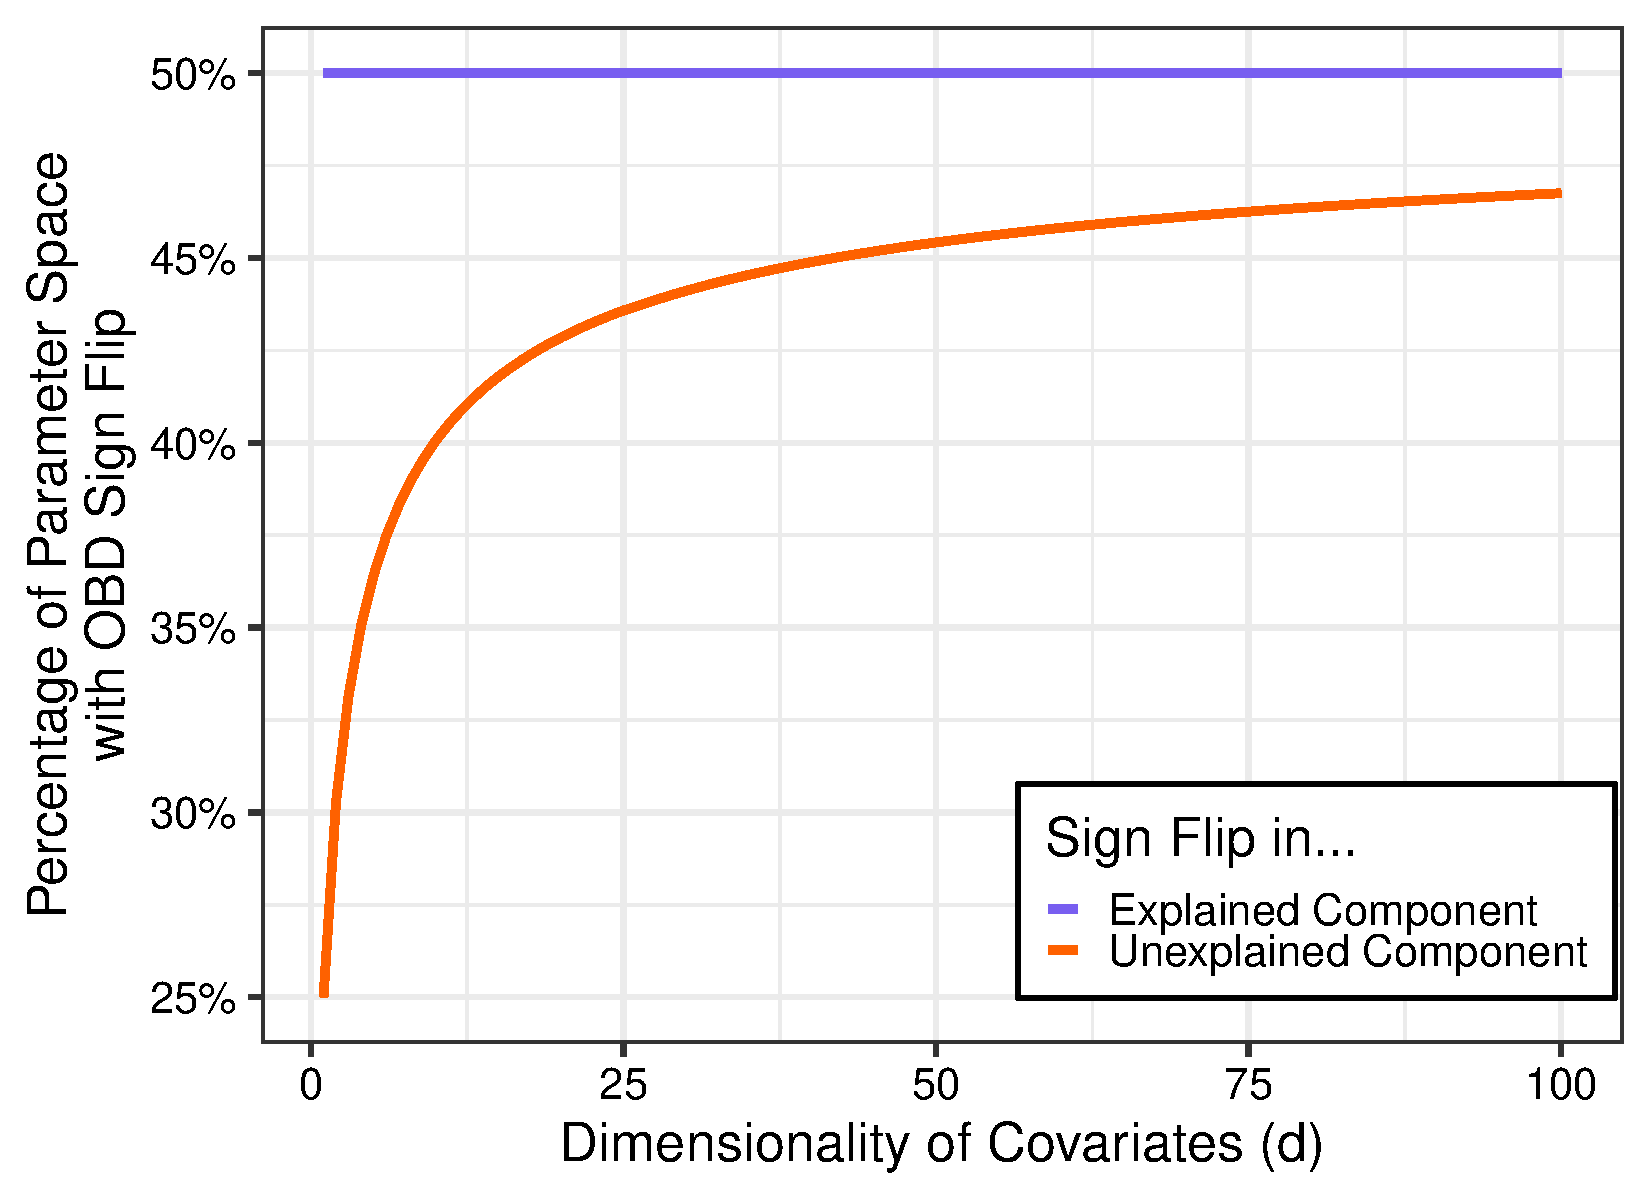
\includegraphics[width=0.75\linewidth]{Sections/Figures/prob_unexplained.pdf}}
    \caption{Percentage of parameter space leading to sign flips. See \cref{remark:computing_irwin_hall} for how we compute the probability for the unexplained component.}
    \label{fig:prob_unexplained}
\end{figure}

\cref{sec:real_example,sec:example} demonstrate that, in practical scenarios, sign flips in the OBD can occur.
%And \cref{thm:explained_ordering_sensitivity} and \cref{thm:ordering_sensitivity} fully describe the conditions under which sign flips occur.
However, it is not obvious how likely sign flips are.
One way to answer this question is to measure the fraction of parameters ($\mu_g, \beta_g, \alpha_g)$ for $g \in \{H,K\}$ that lead to sign flips. As the next two propositions demonstrate, the fraction leading to sign flips is fairly large.
Throughout this section and the next, we will make use of the fact that as long as the (fairly improbable) event of $\mu_H = \mu_K$ does not occur, we can fix the units of the covariates $X$ such that $\mu_K = 0$ and $\mu_K = 1$; see \cref{lemma:units}.
%
\begin{proposition} \label{prop:explained_fraction}
	Assume $\mu_H \neq \mu_K$ elementwise.
	Let $C_M \subset \R^{2d}$ be a cube with side length $2M > 0$ centered at the origin, and suppose $(\beta_K, \beta_H)$ jointly lie in this cube. Let $C_{flip} \subset C_M$ be the settings of $(\beta_H, \beta_K)$ that lead to a sign flip in the explained component.
	Then we may choose units of $X$ such that $\mu_K = 0 \in \R^d$ and $\mu_H = 1 \in \R^d$, and for for any $M > 0$:
	\begin{equation}
		\frac{\mathrm{Volume}(C_{flip})}{\mathrm{Volume}(C_M)} = \frac{1}{2}.
	\end{equation}
I.e., half of the parameter space leads to sign flips in the explained component.
\begin{proof}
    See \cref{proof:explained_fraction}.
\end{proof}
\end{proposition}
%
\begin{proposition} 
\label{prop:unexplained_fraction}
	Assume $\mu_H \neq \mu_K$ elementwise.
	Let $C_M \subset \R^{2d+2}$ be a cube with side length $2M > 0$ centered at the origin, and suppose $(\beta_K, \beta_H, \alpha_K, \alpha_H)$ jointly lie in this cube.
	Let \( I_2 \sim \text{Irwin-Hall}(2) \) and \( J_{2d} \sim \text{Irwin-Hall}(2d) \) be independent random variables.
	Then we may choose units of $X$ such that $\mu_K = 0$ and $\mu_H = 1 \in \R^d$, and
 	the fraction of $C_M$ for which a sign flip occurs in the unexplained component is given by:
\begin{align} \label{eq:unexplained_fraction}
    Pr \left( \{ I_2 > 1 \} \cap \{ J_{2d} < d + 1 - I_2 \}  \right) + \nonumber \\
    Pr \left( \{ I_2 < 1 \} \cap \{ J_{2d} > d + 1 - I_2 \} \right),
\end{align}
 and this quantity approaches $1/2$ as $d \to \infty$.
 \begin{proof}
    See \cref{proof:unexplained_fraction}.
\end{proof}
\end{proposition}
The joint Irwin-Hall probability in \cref{eq:unexplained_fraction} is hard to evaluate analytically, so in \cref{fig:prob_unexplained} we evaluate it numerically for various values of $d$.
We see that for even modest dimension $d$, the fraction of parameter space leading to sign flips exceeds 40\%.

\section{Are sign flips common?}
\label{sec:no_sign_flips}
\cref{sec:sign_flip_fraction} shows that, as a fraction of parameter space, a large number of parameters lead to sign flips.

However, this seems to contradict empirical evidence.
In particular, in \cref{appendix:icu_details,appendix:us_labor_force}, only a small number of problems lead to sign flips.
And, while not all applications of the OBD in the literature report both choices of reference group $g$, many that do show no sign flip \citep{sharafRashad2016} \textcolor{red}{Will: I believe we have citations for this? Having 3 or so would be good to back up this point.}
One explanation for this tension is that the theoretical analysis places a uniform distribution over the linear regression parameters, while true data-generating processes may be non-uniform.

%While \cref{thm:explained_ordering_sensitivity,thm:ordering_sensitivity} characterizes when sign reversals can arise, it is also useful to understand when they do \emph{not} occur. 
%For the explained component, although differences in coefficients can in principle offset differences in covariate means, the most immediate condition under which no sign reversal occurs is when the covariate mean difference loads in the same direction under both reference models.

For the unexplained component, a sign flip intuitively requires the intercept and slope effects to pull in opposite directions across groups. When both move in the same direction, so that the group with higher baseline outcomes also has higher returns to covariates, the unexplained component preserves its sign regardless of the chosen reference group.

We formalize this idea in the following assumption. 

\begin{assumption}[Aligned intercept--slope effects]
\label{ass:no_sign_flip}
\[
    (\mu_H^T \Delta\beta)(\mu_K^T \Delta\beta) > 0 
\quad \text{and}  
\]
\[
    \sign(\Delta\alpha) = \sign(\mu_H^T \Delta\beta) = \sign(\mu_K^T \Delta\beta),
\]
\end{assumption}

\begin{proposition}
    \label{prop:no_sign_flip}
    Under \cref{ass:no_sign_flip}, the unexplained components 
    \( U^{(H)}\) and  \(U^{(K)}\) share the same sign.
\end{proposition}

\begin{proof}
See \cref{proof:no_sign_flip}.
\end{proof}

Under \Cref{ass:no_sign_flip} both unexplained components share the same sign and the OBD cannot exhibit a sign reversal. 
This assumption requires that the group with higher baseline outcomes ($\alpha_g$) also benefits more from the covariates ($\beta_g$) for \(g \in \{H,K\}\).

For example, in terms of the gender wage example introduced in \cref{sec:counterfactual_example}, \cref{ass:no_sign_flip} corresponds to settings where the group earning higher baseline wages ($\alpha_g$) also experiences higher returns to skills and education ($\beta_g$). 
Here, both intercept and slope advantages move in the same direction, so the unexplained component, presents consistent sign between reference groups. 

Similarly, for the SBP--BMI example in \cref{sec:example}, \cref{ass:no_sign_flip} would correspond to a case where the higher-resource group exhibits both a higher baseline SBP and a stronger SBP--BMI relationship than the lower-resource group. However, in the simulated data, the lower-resource group shows a steeper SBP--BMI slope while having a lower baseline, violating \cref{ass:no_sign_flip}.

We can similarly identify conditions under which a sign flip cannot occur in the explained components. 
Recall that, by definition, there is a sign flip in the explained component if $\sign(\Delta\mu^T \beta_H) \neq \sign(\Delta\mu^T \beta_K)$. The following proposition follows immediately:
%
\begin{proposition} \label{prop:no_explained_sign_flip}
	Assume that $\mu_K \neq \mu_H$ elementwise.
	Then we may choose units for $X$ such that there is no sign flip in the explained components if and only if $\sign (\sum_{i=1}^d \beta_{H,i}) \neq \sign( \sum_{i=1}^d \beta_{K,i})$.
\end{proposition}
%
\begin{proof}
See \cref{proof:no_explained_sign_flip}.
\end{proof}
\cref{prop:no_explained_sign_flip} helps us understand why sign flips in the explained component are unusual in the settings considered in this paper.
In both the SBP--BMI example in \cref{sec:example}, it is expected that any subpopulation will have a positive relationship between BMI and SBP; i.e., we expect $\beta_H, \beta_K > 0$ for any choice of $H, K$.

Similarly, \cref{prop:no_explained_sign_flip} helps us see why few of the hospital mortality analyses from \cref{appendix:icu_details} show explained sign flips: while we might expect the same factor to affect in-mortality in men and women with different magnitudes, there is little a-priori reason to think that the same factor will cause mens' mortality to decrease but womens' to increase (or vice-versa).
Indeed, this makes the sign flip in \cref{sec:real_example} even more surprising.
